\PassOptionsToPackage{unicode=true}{hyperref} % options for packages loaded elsewhere
\PassOptionsToPackage{hyphens}{url}
%
\documentclass[ignorenonframetext,aspectratio=43,]{beamer}
\usepackage{pgfpages}
\setbeamertemplate{caption}[numbered]
\setbeamertemplate{caption label separator}{: }
\setbeamercolor{caption name}{fg=normal text.fg}
\beamertemplatenavigationsymbolsempty
% Prevent slide breaks in the middle of a paragraph:
\widowpenalties 1 10000
\raggedbottom
\setbeamertemplate{part page}{
\centering
\begin{beamercolorbox}[sep=16pt,center]{part title}
  \usebeamerfont{part title}\insertpart\par
\end{beamercolorbox}
}
\setbeamertemplate{section page}{
\centering
\begin{beamercolorbox}[sep=12pt,center]{part title}
  \usebeamerfont{section title}\insertsection\par
\end{beamercolorbox}
}
\setbeamertemplate{subsection page}{
\centering
\begin{beamercolorbox}[sep=8pt,center]{part title}
  \usebeamerfont{subsection title}\insertsubsection\par
\end{beamercolorbox}
}
\AtBeginPart{
  \frame{\partpage}
}
\AtBeginSection{
  \ifbibliography
  \else
    \frame{\sectionpage}
  \fi
}
\AtBeginSubsection{
  \frame{\subsectionpage}
}
\usepackage{lmodern}
\usepackage{amssymb,amsmath}
\usepackage{ifxetex,ifluatex}
\usepackage{fixltx2e} % provides \textsubscript
\ifnum 0\ifxetex 1\fi\ifluatex 1\fi=0 % if pdftex
  \usepackage[T1]{fontenc}
  \usepackage[utf8]{inputenc}
  \usepackage{textcomp} % provides euro and other symbols
\else % if luatex or xelatex
  \usepackage{unicode-math}
  \defaultfontfeatures{Ligatures=TeX,Scale=MatchLowercase}
\fi
\usetheme[]{metropolis}
% use upquote if available, for straight quotes in verbatim environments
\IfFileExists{upquote.sty}{\usepackage{upquote}}{}
% use microtype if available
\IfFileExists{microtype.sty}{%
\usepackage[]{microtype}
\UseMicrotypeSet[protrusion]{basicmath} % disable protrusion for tt fonts
}{}
\IfFileExists{parskip.sty}{%
\usepackage{parskip}
}{% else
\setlength{\parindent}{0pt}
\setlength{\parskip}{6pt plus 2pt minus 1pt}
}
\usepackage{hyperref}
\hypersetup{
            pdftitle={Management and analysis of physics datasets, Part. 1},
            pdfauthor={Antonio Bergnoli bergnoli@pd.infn.it},
            pdfborder={0 0 0},
            breaklinks=true}
\urlstyle{same}  % don't use monospace font for urls
\newif\ifbibliography
\usepackage{graphicx,grffile}
\makeatletter
\def\maxwidth{\ifdim\Gin@nat@width>\linewidth\linewidth\else\Gin@nat@width\fi}
\def\maxheight{\ifdim\Gin@nat@height>\textheight\textheight\else\Gin@nat@height\fi}
\makeatother
% Scale images if necessary, so that they will not overflow the page
% margins by default, and it is still possible to overwrite the defaults
% using explicit options in \includegraphics[width, height, ...]{}
\setkeys{Gin}{width=\maxwidth,height=\maxheight,keepaspectratio}
\setlength{\emergencystretch}{3em}  % prevent overfull lines
\providecommand{\tightlist}{%
  \setlength{\itemsep}{0pt}\setlength{\parskip}{0pt}}
\setcounter{secnumdepth}{0}

% set default figure placement to htbp
\makeatletter
\def\fps@figure{htbp}
\makeatother


\title{Management and analysis of physics datasets, Part. 1}
\providecommand{\subtitle}[1]{}
\subtitle{Fifth Laboratory}
\author{Antonio Bergnoli bergnoli@pd.infn.it}
\date{18/12/2019}
\logo{\includegraphics{images/INFNlogo2017.png}}

\begin{document}
\frame{\titlepage}

\begin{frame}
\tableofcontents[hideallsubsections]
\end{frame}
\hypertarget{laboratory-introduction}{%
\part{Laboratory Introduction}\label{laboratory-introduction}}

\begin{frame}{Goals}
\protect\hypertarget{goals}{}

\begin{itemize}
\item
  Become familiar with SPI protocol.
\item
  Serial Flash Memory as SPI slave.
\end{itemize}

\end{frame}

\hypertarget{spi}{%
\part{SPI}\label{spi}}

\begin{frame}{SPI - Wiki}
\protect\hypertarget{spi---wiki}{}

\includegraphics[width=1\textwidth,height=\textheight]{images/spi_1}

\includegraphics[width=1\textwidth,height=\textheight]{images/spi_2}

\end{frame}

\begin{frame}{SPI (1)}
\protect\hypertarget{spi-1}{}

\begin{itemize}
\item
  SPI (Serial Peripheral Interface) :

  \begin{itemize}
  \item
    it is serial: the data is transmitted one bit at a time;
  \item
    it is synchronous: the transmission of the data is imposed by the
    clock;
  \item
    it has an architecture master/slave(s);
  \end{itemize}
\item
  It is a basic serial protocol (not the most).
\item
  It is mostly used for the communication between \(\mathrm{\mu}\)C or
  FPGA and ICs like: A/D, D/A converters, sensors, memories ...
\end{itemize}

\end{frame}

\begin{frame}{SPI (2)}
\protect\hypertarget{spi-2}{}

\includegraphics[width=1\textwidth,height=\textheight]{images/spi_schema}

\begin{itemize}
\item
  The data are exchanged between a master and a slave.
\item
  Essentially each device has inside it a shift register with the data.
  The data transmission "exchanges" the data between the shift
  registers.
\item
  The Master addresses the Slave and it manages the data transmission
  with the clock (on the \textbf{rising edge}).
\end{itemize}

\end{frame}

\begin{frame}{SPI (3) SPI signals (from the slave side):}
\protect\hypertarget{spi-3-spi-signals-from-the-slave-side}{}

\begin{itemize}
\item
  \textbf{CS} or \textbf{SS}: Chip (Slave) Select. When this input
  signal is low, the device is selected.
\item
  \textbf{CLK}: Clock. This input signal provides the timing for the
  serial interface. Instructions, addresses, or data present at the MOSI
  are latched (evaluated) on the rising edge of the clock.
\item
  \textbf{MOSI}: Master Output Slave Input. This input signal is used to
  transfer data serially into the device. It receives instructions,
  addresses, and the data to be programmed.
\item
  \textbf{MISO}: Master Input Slave Output. This output signal is used
  to transfer data serially out of the device.
\end{itemize}

\end{frame}

\begin{frame}{SPI (4)}
\protect\hypertarget{spi-4}{}

\includegraphics[width=0.8\textwidth,height=\textheight]{images/board}

\end{frame}

\hypertarget{serial-flash-memory}{%
\part{Serial Flash Memory}\label{serial-flash-memory}}

\begin{frame}{Flash Memory}
\protect\hypertarget{flash-memory}{}

\includegraphics[width=1\textwidth,height=\textheight]{images/flash}

\end{frame}

\begin{frame}{Flash Memory - Organization}
\protect\hypertarget{flash-memory---organization}{}

\includegraphics[width=1\textwidth,height=\textheight]{images/org}

\begin{itemize}
\item
  \(16777216 = 2^{24}\);
\item
  Therefore the address of each 8-bit register is a 24-bit address.
\end{itemize}

\end{frame}

\begin{frame}{Flash Memory - Read (1)}
\protect\hypertarget{flash-memory---read-1}{}

To read the memory content in SPI protocol different instructions are
available: READ, Fast Read, Dual Output Fast Read, Dual Input Output
Fast Read, Quad Output Fast Read and Quad Input Output Fast read,
allowing the application to choose an instruction to send addresses and
receive data by one, two or four data lines.

\includegraphics[width=1\textwidth,height=\textheight]{images/table}

\end{frame}

\begin{frame}{Flash Memory - Read (2)}
\protect\hypertarget{flash-memory---read-2}{}

\includegraphics[width=1\textwidth,height=\textheight]{images/read}

\end{frame}

\begin{frame}{Flash Memory - Read (3)}
\protect\hypertarget{flash-memory---read-3}{}

\begin{itemize}
\item
  The device is selected by driving the CS low.
\item
  The instruction code for the READ instruction (\(00000011_2\)) is
  sent. Each bit is latched-in (evaluated) on the rising edge of the
  clock.
\item
  The 3 bytes address (23,22,...,1,0) are then sent. Each bit is
  latched-in (evaluated) on the rising edge of the clock.
\item
  Then the memory content, at that address, is shifted out on the MISO,
  each bit is sent, on the falling edge of Serial Clock (C). But
  evaluated by the Master on the following rising-edge.
\item
  The READ instruction is terminated by driving the CS high.
\end{itemize}

\end{frame}

\hypertarget{homework}{%
\part{Homework}\label{homework}}

\begin{frame}{Homework}
\protect\hypertarget{homework-1}{}

\begin{itemize}
\tightlist
\item
  \textbf{You have to write the VHDL code to implement an SPI master, in
  order to read the data stored in a 8-bit register of the serial flash
  memory.}
\end{itemize}

\includegraphics[width=0.5\textwidth,height=\textheight]{images/master}

\end{frame}

\begin{frame}{Hmw - Master signals (1)}
\protect\hypertarget{hmw---master-signals-1}{}

\begin{itemize}
\item
  clock: the clock provided by the oscillator mounted on the evaluation
  board;
\item
  miso;
\item
  reset: provided by the VIO. It is used to reset the FSM;
\item
  start: provided by the VIO. It is used to start the READ operation, on
  the rising edge of the signal;
\item
  txd: a 32 bit signals. It is formed by the the instruction byte and
  the address 3 bytes. The address (or rather the last 4 significant
  bits) is provided by the VIO;
\end{itemize}

\end{frame}

\begin{frame}{Hmw - Master signals (2)}
\protect\hypertarget{hmw---master-signals-2}{}

\begin{itemize}
\item
  cs: when you have received the 8 bits stored in a register, after the
  read operation, the CS has to switch from `0' to `1';
\item
  mosi;
\item
  ready: the ready is a pulse `0' \(\rightarrow\) `1' \(\rightarrow\)
  `0' that happens when you have received the 8 bits stored in a
  register, after the read operation;
\item
  rxd: a 8 bit signals. It is formed by the 8 bits obtained by the read
  operation;
\item
  sclk: is the clock generated by the master, that synchronizes the data
  transmission.
\end{itemize}

\end{frame}

\begin{frame}{Memory Configuration}
\protect\hypertarget{memory-configuration}{}

\begin{itemize}
\item
  The flash memory must be configured using the .mcs file in the folder
  \(flash\_configuration\). With this .mcs file you are going to write
  the first six flash memory locations with these values:

  \begin{enumerate}
  \item
    @ address 0x000000 \(\Rightarrow\) 0x00;
  \item
    @ address 0x000001 \(\Rightarrow\) 0x01;
  \item
    @ address 0x000002 \(\Rightarrow\) 0x02;
  \item
    @ address 0x000003 \(\Rightarrow\) 0x03;
  \item
    @ address 0x000004 \(\Rightarrow\) 0x04;
  \item
    @ address 0x000005 \(\Rightarrow\) 0x05.
  \end{enumerate}
\item
  \textbf{0x} stands for hexadecimal value.
\item
  The configuration of the flash memory using in the .mcs file is
  described in the section 3 of the third laboratory.
\end{itemize}

\end{frame}

\begin{frame}{Hints (1)}
\protect\hypertarget{hints-1}{}

\begin{itemize}
\item
  You can download all the folder \(Lab8\), open the project (the file
  .xpr) and work there.
\item
  You have to write the code \textbf{only} inside the file
  \(spi\_master.vhd\).
\item
  The SPI master can be implemented as a 3 state FSM.
\item
  \textbf{Remember} the testbenches !!!
\end{itemize}

\end{frame}

\begin{frame}{Hints (2)}
\protect\hypertarget{hints-2}{}

You can use this code as an inspirational source for you code. It is a
\textbf{partial} implementation of a state of the FSM. In particular in
this state the txd word is transmitted to the slave.

\includegraphics[width=1\textwidth,height=\textheight]{images/code}

\end{frame}

\begin{frame}{Hints (3)}
\protect\hypertarget{hints-3}{}

It might be very useful exploit the ILA core(s) in order to monitor the
state of the FSM, the internal signals and the signals representing the
SPI master inputs and output.\\
\textbf{For the final check instantiates an ILA core, where you monitor
the CS, the MOSI, the MISO and the SCLK. You must get a temporal diagram
very similar to the diagram of the picture/ slide 15.} Monitor also the
"ready" signal.

\includegraphics[width=1\textwidth,height=\textheight]{images/ila}

\end{frame}

\end{document}
